\subsection{Exploring the Cheerful Waves: Antenna Fun Below Resonance!}

\begin{tcolorbox}[colback=gray!10, colframe=black, title=E9D10] How does radiation resistance of a base-fed whip antenna change below its resonant frequency?

\begin{enumerate}[label=\Alph*.]
    \item Radiation resistance increases
    \item \textbf{Radiation resistance decreases}
    \item Radiation resistance becomes imaginary
    \item Radiation resistance does not depend on frequency
\end{enumerate} \end{tcolorbox}

\subsubsection{Conceptual Background}

To understand the change in radiation resistance of a base-fed whip antenna below its resonant frequency, we must first consider what radiation resistance is. Radiation resistance is a component of the total resistance that an antenna presents to the transmitter, which is associated with the radiation of electromagnetic waves. It is an essential parameter to determine the efficiency of the antenna.

An antenna resonates at a specific frequency, where its impedance is purely resistive. Below this resonant frequency, the antenna behaves differently due to its reactive component. When the frequency drops below resonance, the antenna becomes inductively reactive.

\subsubsection{Mathematical Explanation}

To analyze the behavior of radiation resistance with frequency, we can refer to the basic principles governing antennas. As the frequency decreases:
- The inductive reactance (\(X_L\)) increases.
- The impedance (\(Z\)) seen at the feed point is given by:
\[
Z = R + jX
\]
where \(R\) is the radiation resistance and \(X\) is the reactance which is positive (inductive). 

As the frequency decreases, the following approximations apply for a short antenna:
- The radiation resistance \(R\) is typically lower at these frequencies because the antenna is not effective in radiating energy at low frequencies. This can be represented by the following relation:

\[
R \propto \frac{f^2}{\lambda^2}
\]
where \(f\) is the frequency and \(\lambda\) is the wavelength.

Since \(\lambda = \frac{c}{f}\), where \(c\) is the speed of light (\(c \approx 3 \times 10^8 \, \text{m/s}\)), we can further express \(R\) as:
\[
R \propto \frac{f^2}{\left( \frac{c}{f} \right)^2} = \frac{f^4}{c^2}
\]
This shows that as frequency \(f\) decreases, the radiation resistance \(R\) also decreases.

\subsubsection{Conclusion}

In conclusion, 

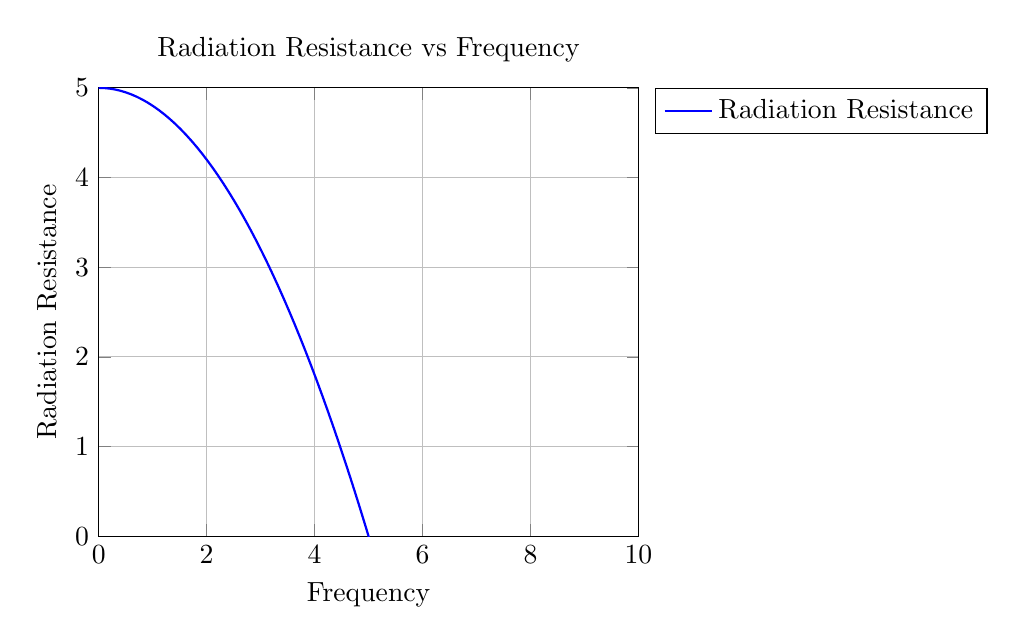
\begin{tikzpicture}
    \begin{axis}[
        xlabel={Frequency},
        ylabel={Radiation Resistance},
        grid=both,
        title={Radiation Resistance vs Frequency},
        legend pos=outer north east,
        xmin=0, xmax=10,
        ymin=0, ymax=5,
        samples=100,
        domain=0:10,
    ]
    \addplot[blue, thick] {5 - (x^2)*0.2}; % hypothetical curve
    \addlegendentry{Radiation Resistance}
    \end{axis}
\end{tikzpicture}
